\documentclass[_main.tex]{subfiles}
 
\begin{document}

\section*{Genetic variation at a haplotype locus} \label{main_haplo}

We need to take account of recombination as well as mutation at a haplotype locus (see glossary figure \ref{fig:supp_graph_17}).  For a locus spanning hundreds of kilobases, the rates of recombination and mutation may be so high that it is rare for two alleles to have the same haplotype, i.e. the same DNA sequence.  Let $G_L$ be the probability that two alleles have the same DNA sequence at a haplotype locus of length $L$.  We call this \textit{haplotype homozygosity} and we would like to be able to estimate its value for any combination of transmission parameters.

\paragraph{Locus scaled recombination rate $r$.}  Let $r$ be the rate of recombination at a haplotype locus, scaled by its length in kilobases.   For a locus of length $L$ kilobases, the probability of recombination occurring within the locus during one generation of transmission is $rL$.

\textit{Plasmodium} parasites reproduce asexually for most of their life cycle but shortly after entering a mosquito vector they undergo sexual mating, with the result that recombination occurs exactly once per generation of host to host transmission.  The rate of recombination between two point loci is conventionally expressed in centimorgans, where 1 centimorgan denotes 1\% probability of recombination per generation.  From experimental genetic crosses it has been estimated that 1 centimorgan is equivalent to $13.5$ kilobases when averaged across the \textit{P. falciparum} genome \cite{Miles2016}.  From this we obtain an estimate of $r = 7.4 \times 10^{-4}$ per kilobase per generation.

\paragraph{Locus scaled mutation rate $v$.}  Let $v$ be the rate of mutation at a haplotype locus, scaled by its length in kilobases.   For a locus of length $L$ kilobases, the probability of a mutation occurring within the locus during one generation of transmission is $vL$.

To estimate $v$ we must consider all types of mutation that might alter the DNA sequence of a haplotype locus.  \textit{P. falciparum} has a very high rate of indel mutation, estimated by laboratory studies \textit{in vitro} to be $\sim 2 \times 10^{-9}$ per nucleotide per 48 hour erythrocytic growth cycle \cite{Hamilton2016}.  This is much greater than the single nucleotide substitution rate, but these indel mutations occur mainly within short tandem repeat sequences, so they probably include many recurrent mutations and reversions.  Other types of mutation, such as large copy number variations and structural variations, are much less common.  In principle we could assign different values to $v$ depending on genomic location, since short tandem repeat sequences and indel mutations are concentrated largely in non-coding regions, but for present purposes we shall assume that the mutation rate is constant across the genome and across the life cycle.  If we take the rate of indel mutations plus single nucleotide substitutions to be $10^{-9}$ per nucleotide per day, and if we assume a serial interval of $\tau = 3$ months, we obtain an estimate of $v = 9 \times 10^{-5}$ per kilobase per generation.

\paragraph{Inaccessible regions of the parasite genome.}  Here we focus on haplotype loci within the `core' \textit{P. falciparum} genome which excludes the sub-telomeres and a few other regions that are extremely difficult to sequence using short-read technologies because of their exceptionally complex patterns of polymorphism \cite{Miles2016}.  These hypervariable regions contain genes involved in immune evasion that undergo frequent structural rearrangements by means of a specialised mutational process called non-allelic homologous recombination \cite{Claessens2014}.  Highly mutable genes could in theory be extremely informative about transmission dynamics, but for present purposes we treat them as inaccessible to haplotypic analysis because they cannot be reliably ascertained in field samples with current methodologies. 

\paragraph{Determinants of haplotype homozygosity.}  
\label{main_haplotype_homozygosity} What is the expected homozygosity of a haplotype locus of length $L$?  To address this question, let us randomly sample two alleles from the parasite population and call them alleles 1 and 2.  We randomly select a single nucleotide position within our haplotype locus and call it point A.  Let $\text{A}_1$ and $\text{A}_2$ be the lineages corresponding to alleles 1 and 2 at point locus A.  Let \textbf{T} be a random variable representing time to coalescence of the $\text{A}_1$ and $\text{A}_2$ lineages.   Time to coalescence can vary across a haplotype locus (figure \ref{fig:diff_lineage}) but, as long as the probability distribution of time to coalescence is the same for every point locus, for the following calculations it does not matter where point A is situated within our haplotype locus.

\begin{figure}[h!]
\centering
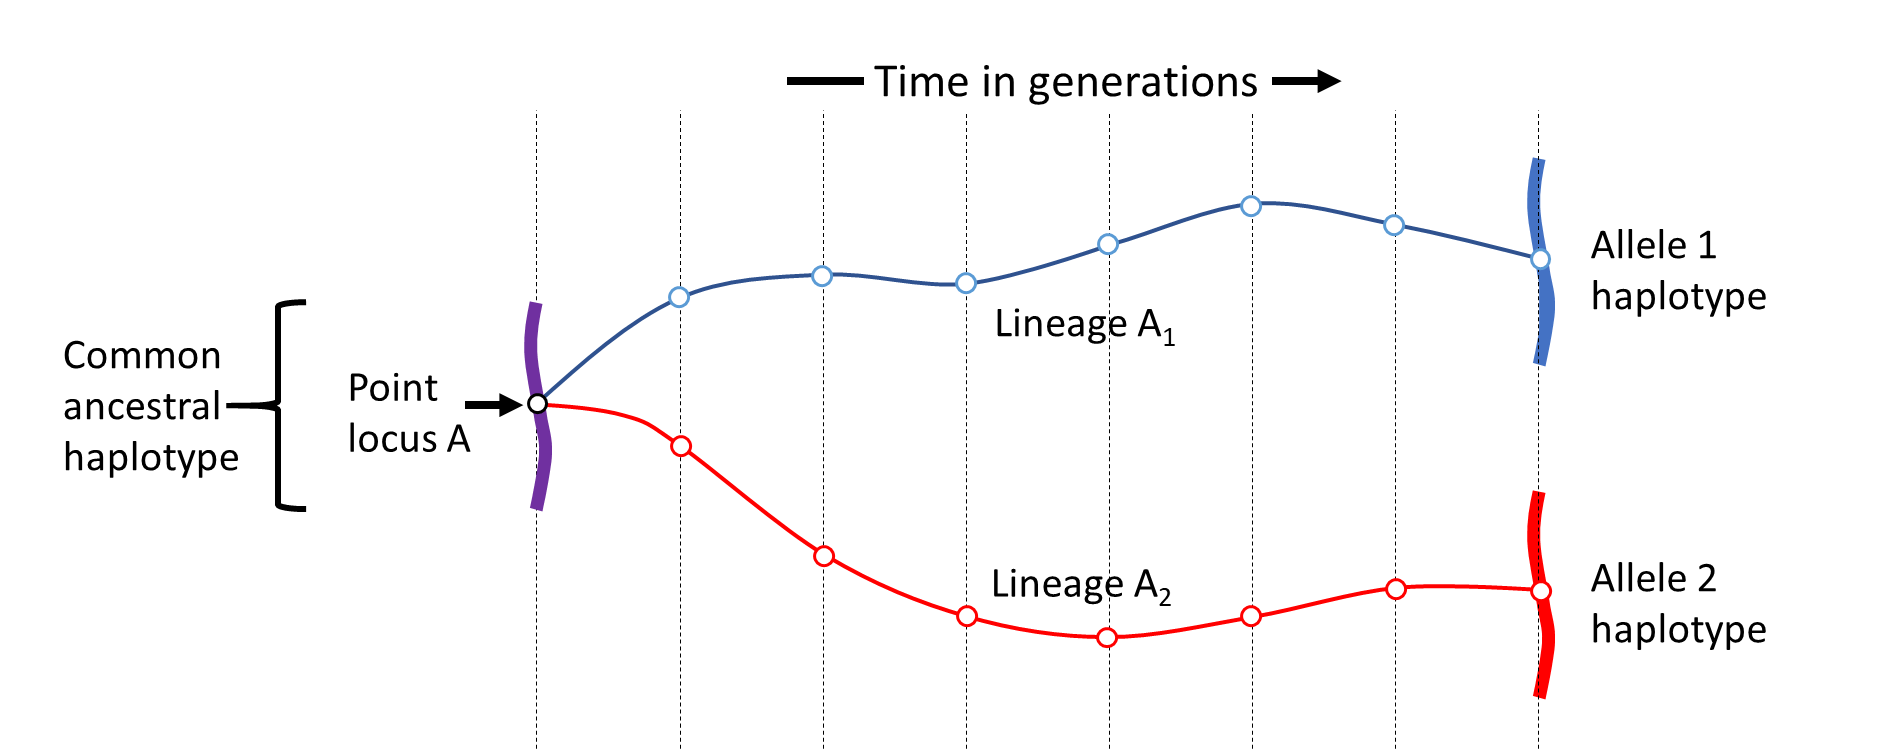
\includegraphics[width=12cm]{181003_hap_lineages.png}
%201215_haplotype.png}
\caption{\textbf{Illustration of the principle of haplotype homozygosity.}  We imagine a haplotype locus of length $L$ kilobases and a point locus A (open circle) somewhere within this haplotype locus.  We sample two alleles at point locus A and trace their lineages back in time until they coalesce in a common ancestral haplotype.  Haplotype homozygosity is the probability that the haplotype locus will be unaffected by recombination or mutation in the time that it takes for the two lineages to coalesce.}
\label{fig:main_ancestral_haplotype}
\end{figure}

By definition, the $\text{A}_1$ and $\text{A}_2$ lineages coalesce when they meet in the same ancestral parasite, whose DNA sequence we will call their \textit{common ancestral haplotype} (figure \ref{fig:main_ancestral_haplotype}). We are interested in what happens to this common ancestral haplotype over the course of $\textbf{T}$ generations between the time of sampling our two alleles and the time of coalescence.  If we track the haplotype associated with either the $\text{A}_1$ or the $\text{A}_2$ lineage over time, in each generation there is a probability of $vL$ that it will be affected by mutation and of $rL$ that it will experience recombination.   

Recombination will change the DNA sequence of the haplotype in some circumstances but not others, e.g. it might not do so if the recombining parasites are siblings and have identical haplotypes at this locus.  We are interested in the frequency of \textit{effective recombination} which we define as recombination between genetically distinct alleles that acts to change the DNA sequence of the haplotype locus.  Suppose that recombination occurs at time $t$ and let $\phi_t$ be the probability that this recombination event results in a change to the DNA sequence of this locus.  This means that the probability of effective recombination is $\phi_t r L$ and the probability that the haplotype remains unchanged over the course of one generation is $ ( 1 - v L - \phi_t r L )$. 

By following both lineages over $\textbf{T}$ generations to their point of coalescence, we can obtain the probability that alleles 1 and 2 have retained the common ancestral haplotype, which gives us the probability $G_L$ that the alleles are homozygous at this haplotype locus.

\begin{equation*}
G_L = \prod_{t=1}^\textbf{T}(1 - v L - \phi_t r L )^2
\end{equation*}

We obtain the expectation of haplotype homozygosity by summation across the probability distribution of coalescence times:

\begin{equation}
E \{ G_L \} = \sum_{i=1}^\infty \Pr \{ \textbf{T} = i \} \prod_{t=1}^i (1 - vL - \phi_t rL)^2
\label{eq:main_G_L_mean} 
\end{equation}

\paragraph{Effective recombination parameter $\phi_t$.} We are left with the question of how to estimate $\phi_t$ which we call the \textit{effective recombination parameter}.   In order for sexual recombination to change the DNA sequence of a haplotype, it is necessary for the mating parasites to be heterozygous at that locus.  We could therefore say that $\phi_t$ is equivalent to the probability that the mating parasites are heterozygous, which is given by the value  of within-host heterozygosity $H_W$ at that locus at time $t$.  However this assumes random mating (i.e. that a vector randomly samples parasites from a host, and that these randomly mate within the vector) whereas a number of empirical studies have found evidence of mating bias and a tendency to selfing.  Another complication is that the recombination of two heterozygous haplotypes might not result in a new haplotype if their DNA sequences are similar, especially if the recombination breakpoint is away from the centre of the locus. Therefore we shall say that 

\begin{equation}
\phi_t = f \widehat{H}_W
\label{eq:main_phi} 
\end{equation}

where $\widehat{H}_W$ is the mean level of within-host heterozygosity in the population at time $t$, and $f$ is a factor that we use to correct for mating bias and other causes of non-effective recombination.  The value of $f$ is in the range [0,1] where $f=1$ indicates that there is no mating bias and that the recombination of two heterozygous haplotypes always results in a new haplotype.

It will be evident from equations \ref {eq:main_G_L_mean} and \ref{eq:main_phi} that evaluation of haplotype homozygosity at a particular point in time requires knowledge of within-host heterozygosity at multiple previous time points, i.e. this is a non-Markovian process.  We use a heuristic approach to solve this problem.  We start by assuming some arbitrary value for $\widehat{H}_W$ in the distant past and then progressively construct a time series of $\widehat{H}_W$ values by forwards-in-time simulation, pausing to perform backwards-in-time Markovian simulation of coalescence times for each new timepoint.

%%%%%%%%%%%%%%%%%%%%%%%%%%%%%%%%%%%%%%

\paragraph{Relationship of haplotype homozygosity to haplotype length.}  Using the above principles we can determine the expected haplotype homozygosity for a locus of any given length.   Figure \ref{fig:main_hap_hom_vs_length} shows how haplotype homozygosity falls away rapidly as haplotype length increases.  Levels of haplotype homozygosity are much higher if we sample alleles from the same host compared to sampling from different hosts, as we would expect.  Here we see that haplotype homozygosity declines as population size and the rate of superinfection increase, but there can be long stretches of haplotype homozygosity in within-host samples when there is no superinfection. 

\begin{figure}[h!]
\centering
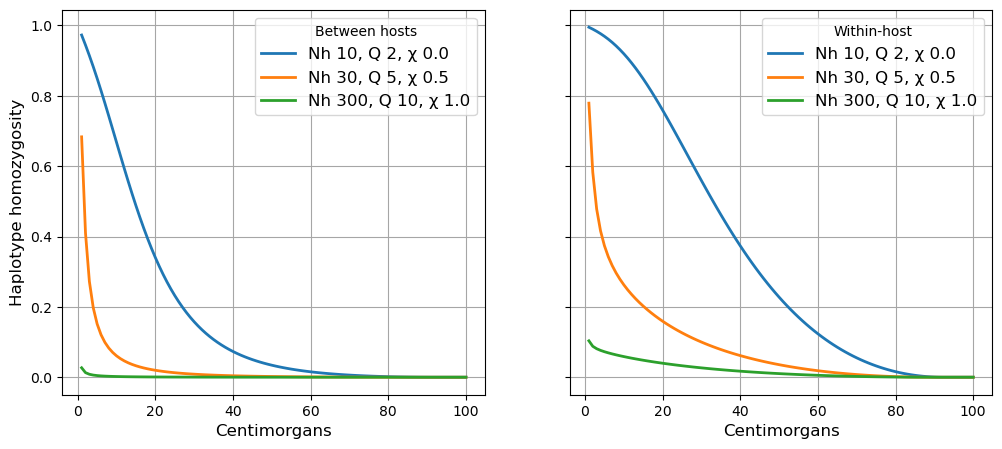
\includegraphics[width=14cm]{230216_hap_hom_vs_length.png}
\caption{\textbf{Relationship between haplotype homozygosity and haplotype length.} Left panel shows between-host variation (i.e. two alleles sampled from different hosts), right panel shows within-host variation (i.e. two alleles sampled from the same host).  \href{https://d-kwiat.github.io/gtg/haplotype-homozygosity.html}{See worked example.}
} 
\end{figure}

%%%%%%%%%%%%%%%%%%%%%%%%%%%%%%%%%%%%%%

\paragraph{Shared haplotype segments, recent common ancestry and identity by descent.}  \label{main_shs_ancestry}

If we compare the genome sequences of two parasites, we can identify segments of the genome where their haplotypes are identical.  We call these \textit{shared haplotype segments}.  Unrelated parasites often have some shared haplotype segments that extend over a few kilobases, but if we observe a substantial number of shared haplotype segments that are hundreds of kilobases long, this suggests that the parasites share a recent common ancestor. 

Identity by descent (IBD) is a population genetic term that refers to genome sequences that are identical between individuals due to recent common ancestry \cite{Browning2012}.  There are various methods to estimate levels of IBD for \textit{P. falciparum} using whole genome sequence data \cite{Schaffner2018,Henden2018} or genetic barcodes such as SNP panels, microsatellites and microhaplotypes \cite{Taylor2017,Taylor2019,Taylor2020,Gerlovina2022}.  A commonly used metric of genetic relatedness between individuals is the proportion of the genome that is IBD. 

A rather simplistic view of whole genome IBD methods is that they detect shared haplotype segments of above a certain size, typically around 2 centimorgans.   In general we are more likely to observe recent common ancestry and high levels of IBD if the parasite population size is small.  This raises the question of what is the expected proportion of the genome that is IBD for a given set of transmission parameters.

As shown in Methods section \ref{supp_shs} the proportion of the genome occupied by shared haplotype segments of $>k$ centimorgans can be crudely approximated by $E \{G_k \}$, the expected haplotype homozygosity of a locus of $k$ centimorgans.  Thus if we define shared haplotype segments of $>2$ centimorgans as IBD, then the proportion of the genome that is IBD is approximated by the mean homozygosity of a haplotype locus of 2 centimorgans.

Let $\gamma$ be the mean haplotype homozygosity of a 2 centimorgan locus, which corresponds to 27 kilobases if we assume that 1 centimorgan is equivalent to approximately 13.5 kb on average.  Figure \ref{fig:main_hap_hom_27} shows how $\gamma$ varies with different transmission parameters, where $\gamma_S$ represents the local subpopulation and $\gamma_W$ the within-host population.  $\gamma_S$ declines rapidly with increasing levels of $N_h$, $\chi$ and $Q$.  In the absence of superinfection, $\gamma_W$ is high and independent of $N_h$. 

\begin{figure}[h!]
\centering
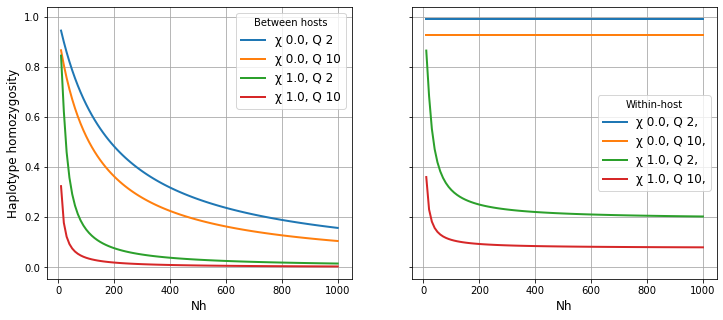
\includegraphics[width=14cm]{221107_hap_hom_27.png}
\caption{\textbf{Haplotype homozygosity of a 2 centimorgan locus.} This metric, denoted $\gamma$, is approximately equal to the proportion of the genome that is identical by descent (IBD) between individuals randomly sampled from a population, as discussed in the main text and Methods section \ref{supp_shs}.  Left panel shows $\gamma_S$ (comparing two alleles sampled from different hosts in the local subpopulation), right panel shows $\gamma_W$ (comparing two alleles sampled from the same host).   \href{https://d-kwiat.github.io/gtg/ibd.html}{See worked example.}}
\label{fig:main_hap_hom_27}
\end{figure}

%\begin{figure}[h!]
%\centering
%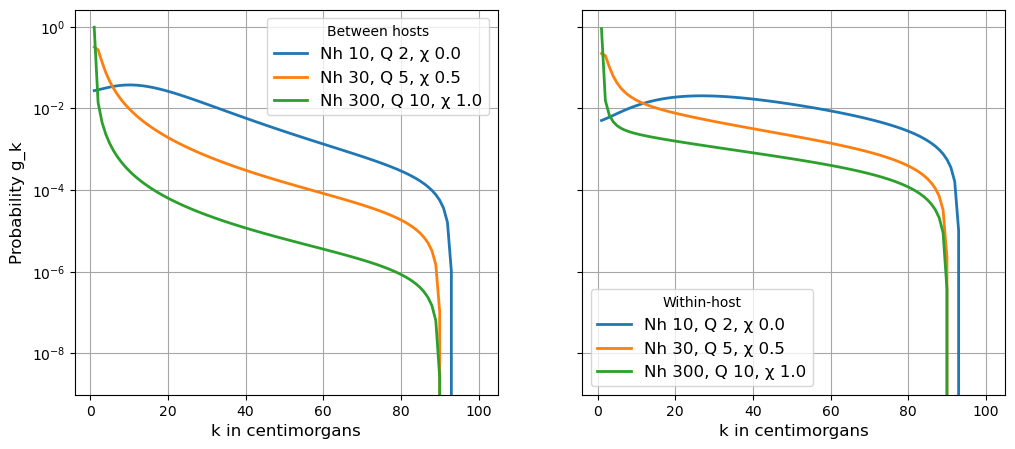
\includegraphics[width=14cm]{230203_shs.png}
%\caption{\textbf{Relationship between $g_k$ and haplotype length.} $g_k$ is the probability that a haplotype of length between $k-1$ and $k$ centimorgans is a shared haplotype segment with respect to two randomly sampled alleles.  Left panel shows between-host variation (i.e. two alleles sampled from different hosts), right panel shows within-host variation (i.e. two alleles sampled from the same host).   \href{https://github.com/d-kwiat/gtg/blob/main/haplotype_homozygosity_vs_length.ipynb}{View code}}
%\label{fig:main_shs_vs_length}
%\end{figure}

\end{document}